\section{Supplementary Material}
\beginsupplement

\begin{figure}[H]
  \centering
  \fbox{
   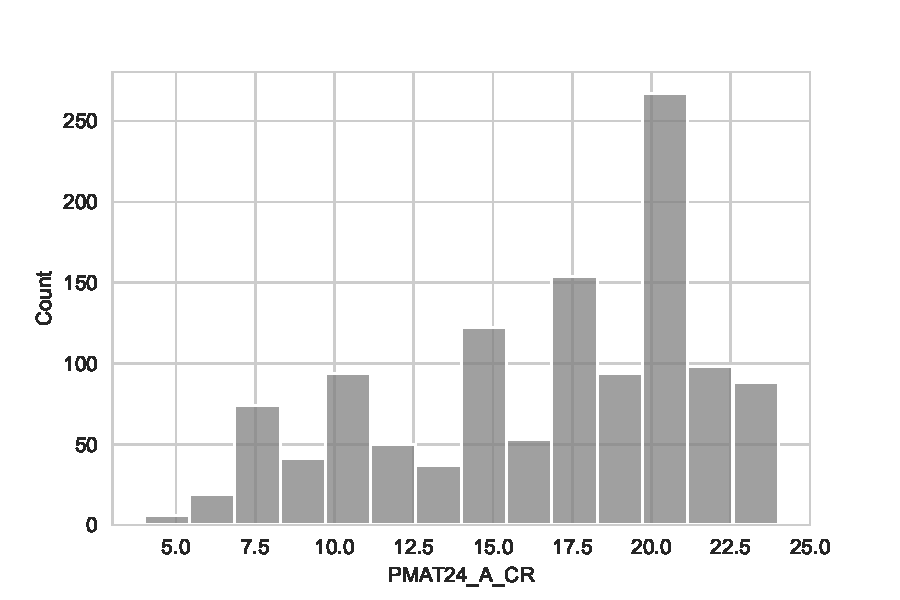
\includegraphics[width=0.36\paperwidth]{fig/supplement/hcp_iq_nonnorm_hist.pdf}
   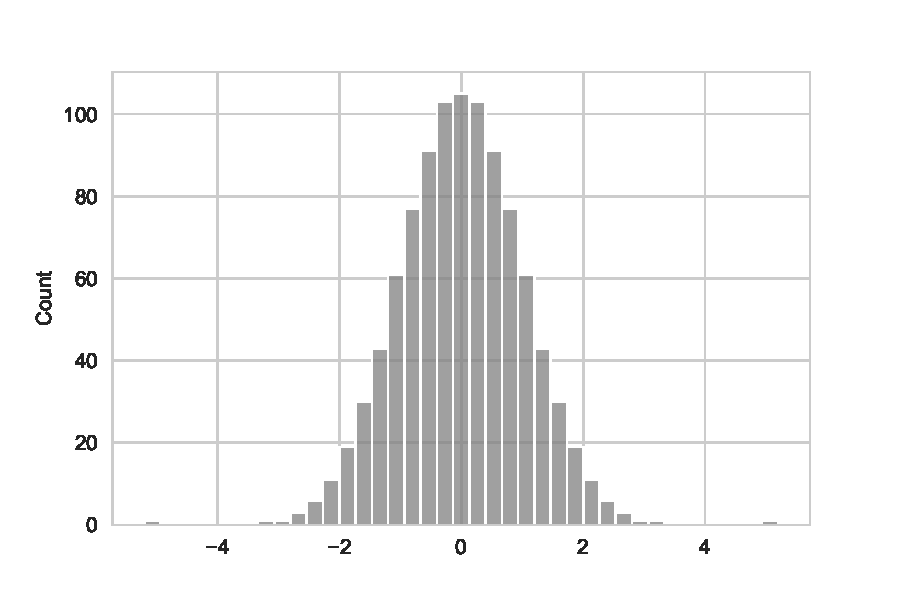
\includegraphics[width=0.36\paperwidth]{fig/supplement/hcp_iq_quanttrf_hist.pdf}
   }
  \caption{Histogram of fluid intelligence score in the HPC dataset, before (left) and after (right) quantile transformation.}
  \label{fig:hcp-hist}
\end{figure}

\begin{figure}[H]
  \centering
  \fbox{
   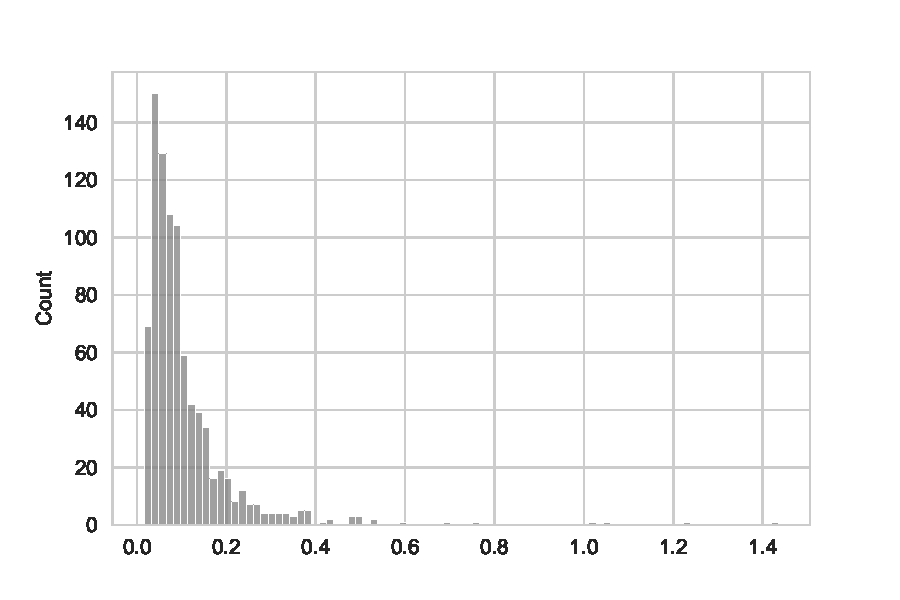
\includegraphics[width=0.36\paperwidth]{fig/supplement/abide_motion_hist.pdf}
   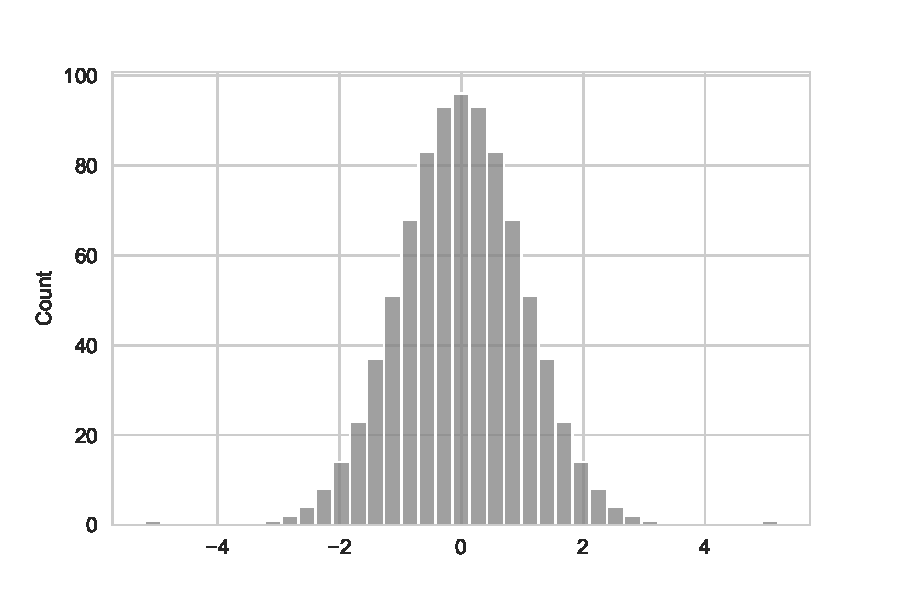
\includegraphics[width=0.36\paperwidth]{fig/supplement/abide_motion_quanttrf_hist.pdf}
   }
  \caption{Histogram of mean framewise displacement in the ABIDE dataset, before (left) and after (right) quantile transformation.}
  \label{fig:abide-hist}
\end{figure}

\begin{figure}[H]
  \centering
  \fbox{
   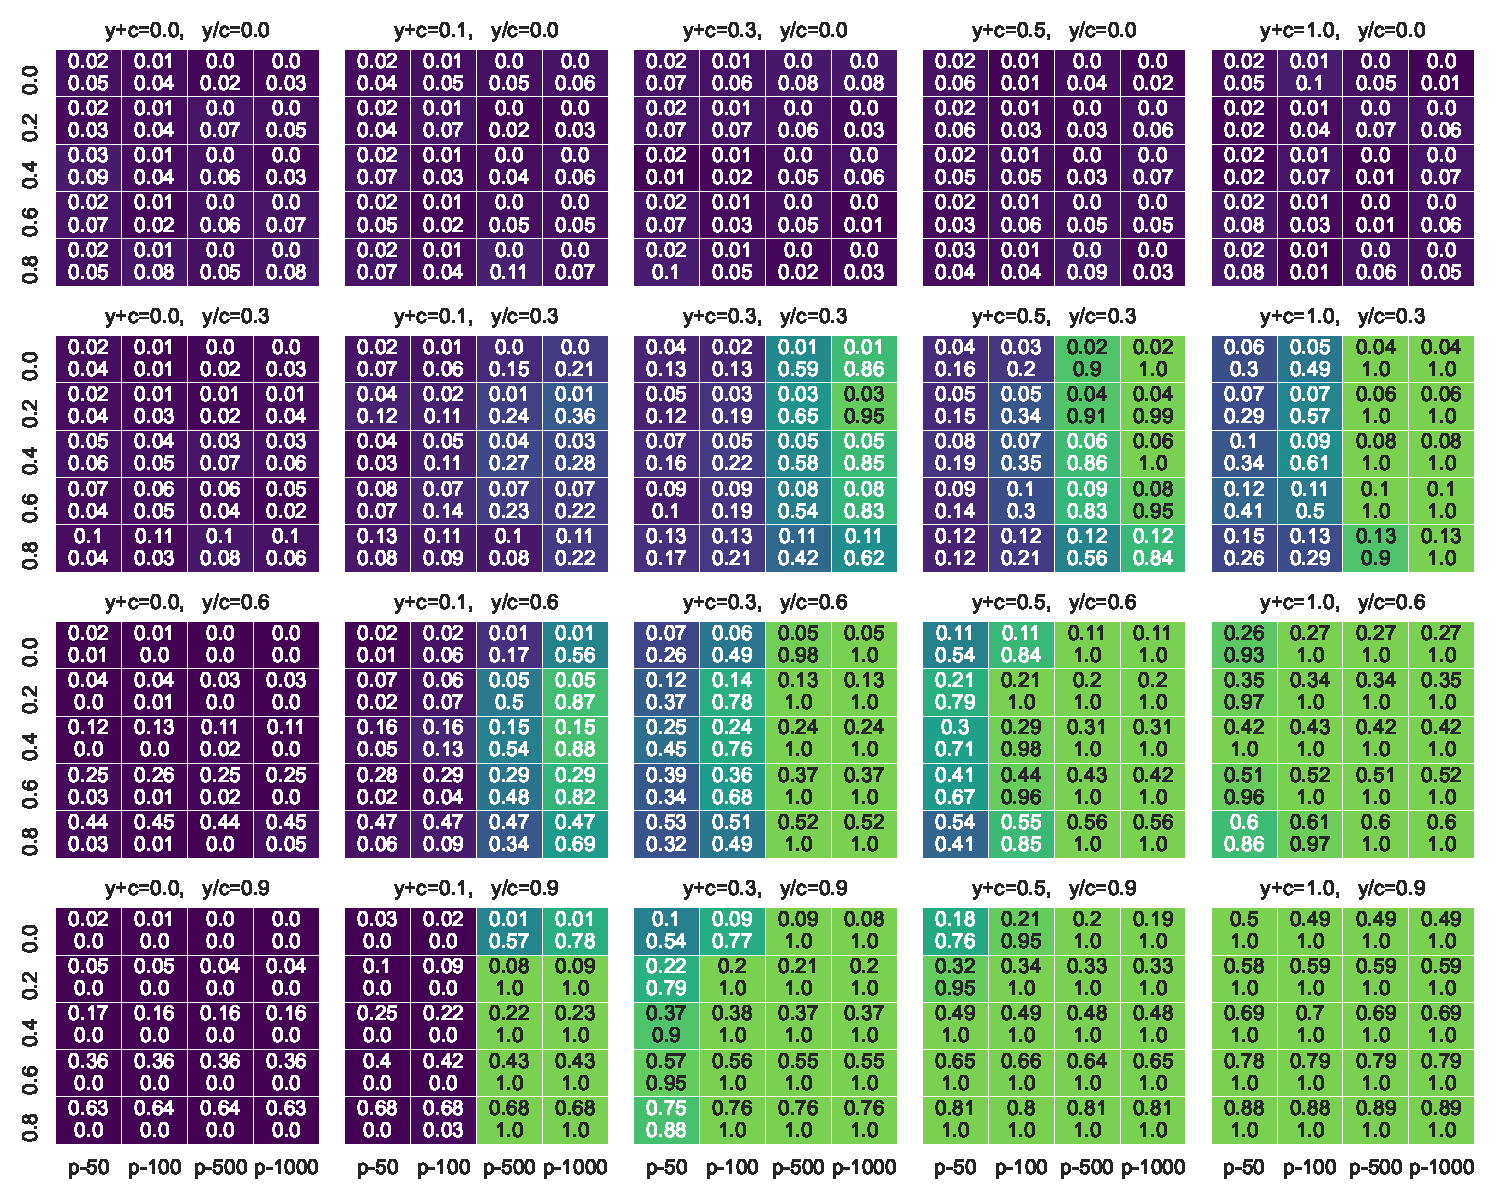
\includegraphics[width=0.75\paperwidth]{fig/supplement/sim_ccc_full_normal_all_heatmap.pdf}}
  \caption{Heatmaps showing the positive rates of the 'full' confounder test, with normally distributed numerical simulated variables.}
  \label{fig:sim-ccc-full}
\end{figure}


\begin{figure}[H]
  \centering
  \fbox{
   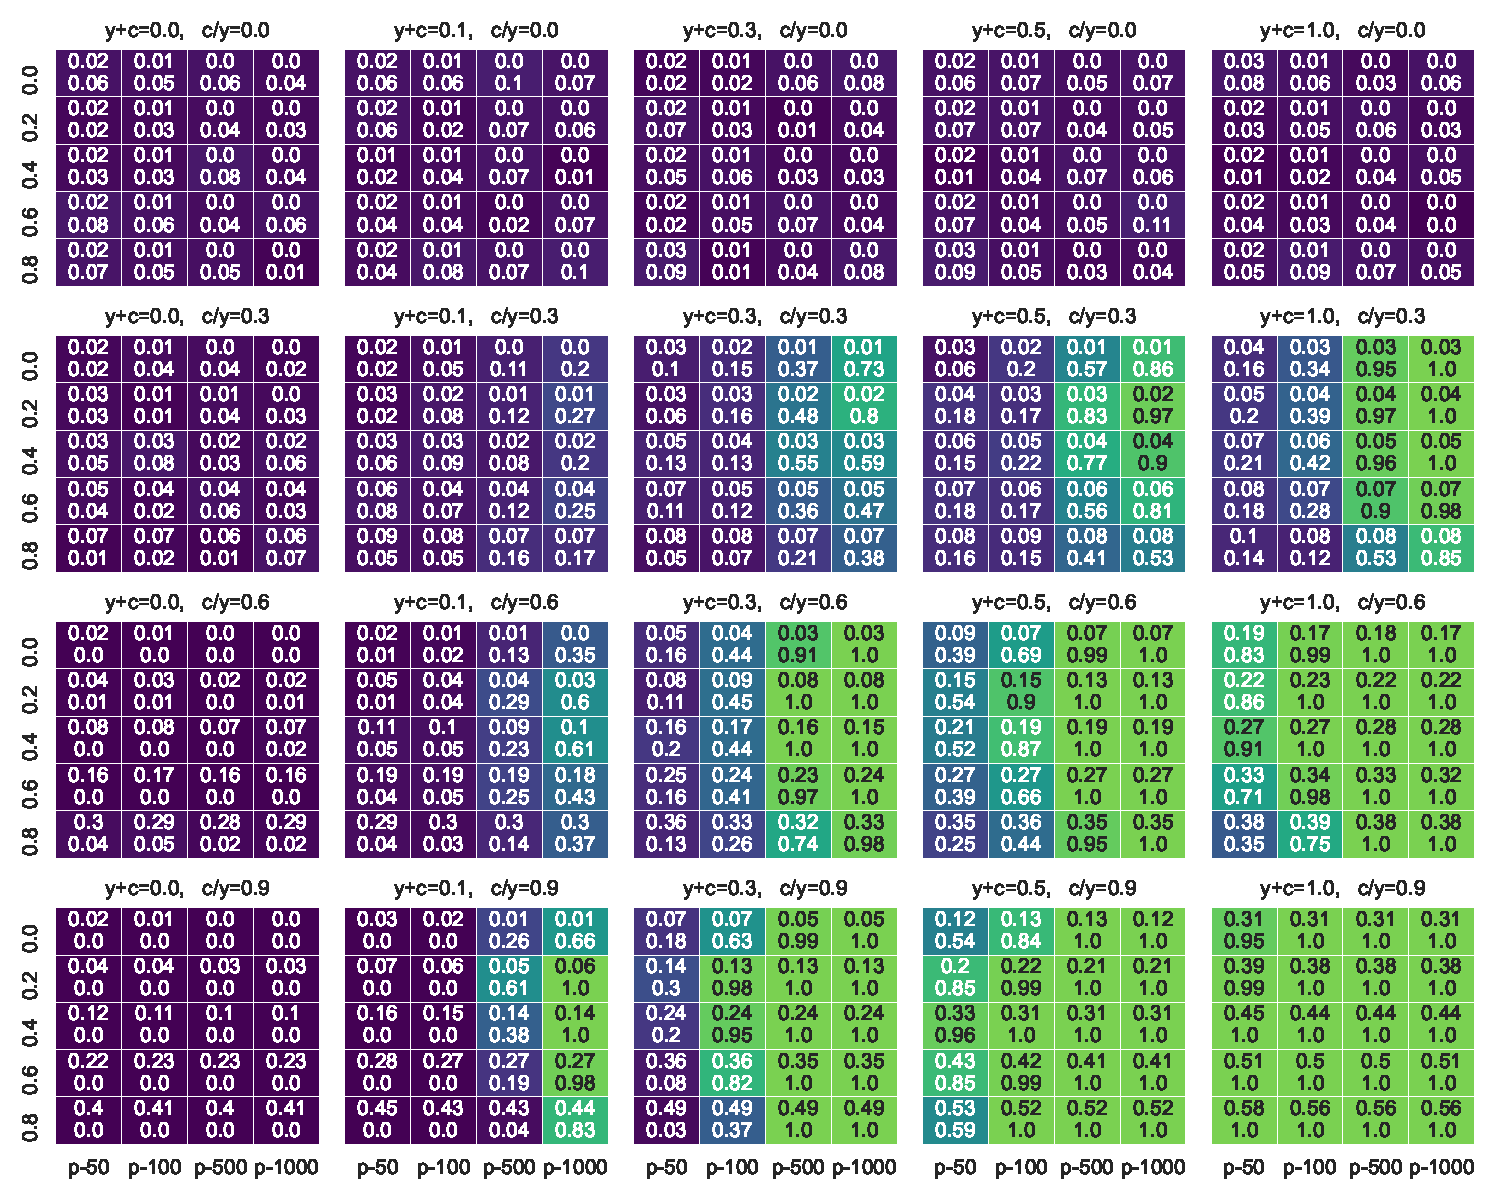
\includegraphics[width=0.75\paperwidth]{fig/supplement/sim_ccb_partial_normal_all_heatmap.pdf}}
  \caption{Heatmaps showing the positive rates of the 'partial' confounder test, with normally distributed numeric $Y$ and $\hat{Y}$ and categorical $C$.}
  \label{fig:sim-ccb-partial}
\end{figure}